\section{技术难点和性能优化}
\subsection{技术难点}
\subsubsection{多语言支持}
\p{
    为了给全球的用户提供方便,我将默认的语言设置成了英语。但是,我在中国,而中文作为世界上使用人数最多的语言,应该也要提供对中文的支持。所以我做了多语言的支持。
}
\p{
    具体的方案是在不同的语言环境(设备默认语言,用户设置语言)下显示不同的文字,就可以考虑在源文件只保存标记,比如\lstinline|i18n.hello|,在加载的时候,根据用户语言的不同,加载不同的语言文件,替换掉原来的标记。比如在\lstinline|en-US|环境下,可以有\lstinline|hello: "Hello"|,在\lstinline|zh-CN|环境下,可以有\lstinline|hello: "你好"|。这样子可以做到不同语言环境显示的语言不同。
}
\p{
    但是,有时候,要渲染的文本中有其他的数据,比如说以下语句:\lstinline|You have 10 seconds left. (en-US)|;\lstinline|你还剩10秒时间 (zh-CN)|。英语和汉语的表达方式和语序有些差异,不能单纯这么拼接。
}
\p{
    这时就要考虑使用模板插值,在语言文件中把要填的数据写成标记,在根据语言渲染文字的时候获得数据,把标记替换成数据,这样就能够保证语序正常又能显示数据。按上面的例子,英语的语言文件中可以这么定义:\lstinline|test: "You have [[ time ]] seconds left."|,中文的语言文件中这么定义:\lstinline|test: "你还剩[[ time ]]秒时间。"|,这中间的\lstinline|time|就是插值的标记,渲染的时候就传入数据
}
.\\
\begin{lstlisting}[language=C++]
    {
        "time": 10
    }
\end{lstlisting}
替换掉标记。
\p{
    可以考虑使用正则表达式匹配标记,例如上文的\lstinline|[[ ]]|就用
}
.\\
\begin{lstlisting}
    /\[\[.+?\]\]/g
\end{lstlisting}
\p{
    最外面的一层\lstinline|/ /g|是声明这是个正则表达式,全局匹配。\lstinline|\\[\\[|匹配前两个方括号。中间的"\lstinline|.|"表示匹配除换行符外的一切字符,\lstinline|+?|表示匹配数量一个及以上,尽可能少匹配,否则有多个插值的话就会匹配成第一个左方括号到最后一个右方括号。\lstinline|\\]\\]|匹配后两个方括号。
}
\p{
    为了让代码更美观一点,方括号之间的空格可写可不写,我们就需要把匹配出来的插值标记的值删去开头两个、末尾两个(去掉方括号)后清除掉前后的空格。最后根据提供的数据替换文本就可以了,下面是最终的源代码。
}
.\\
\begin{lstlisting}
    template(key, arg) {
        let sourceString = map[key];
        const templateMatchRegExp = /\[\[.+?\]\]/g;
        const templates = Array.from(sourceString.matchAll(templateMatchRegExp));
        templates.forEach(match => {
            const src = match[0].slice(2, -2).trim();
            if (arg[src]) {
                sourceString = sourceString.replace(match[0], arg[src].toString());
            } else return;
        });
        return sourceString;
    } 
\end{lstlisting}

\subsubsection{多行文本命令}
\p{
    上文提到,命令处理的时候是按行切割的,这意味着文本命令也只能写在一行内,中间通过\lstinline|\\\\|进行换行。对于换行多的文本编辑、阅读起来就很不方便。为此,我设计了一个宏,支持多行文本命令的编辑,在预处理阶段会将多行文本转换成一行进行编译。如下
}
.\\
\begin{lstlisting}
    text rwd 0.5 0.5 `
    Hello World
    $x^2+y^2=z^2$
    `
\end{lstlisting}
等同于
\begin{lstlisting}
    text rwd 0.5 0.5 Hello World $\\$ $x^2+y^2=z^2$
\end{lstlisting}
渲染效果如下\\
\textbf{Hello World \\ $x^2+y^2=z^2$}
\p{
    可以考虑使用DFA,先扫描把在\lstinline|`|之间的宏标记出来,如下图
}
.\\\\
\begin{tikzpicture}[node distance=150pt]
    \node[draw, rounded corners, fill=green] (normal) {命令};
    \node[draw, rounded corners, right=of set, fill=green] (macro) {多行字符串宏};

    \node[draw, rounded corners, left=50pt of normal, fill=blue] (s1) {};
    \node[draw, rounded corners, below=25pt of s1, fill=blue] (s2) {};
    \node[draw, rounded corners, below=20pt of normal, fill=blue] (s3) {};

    \node[draw, rounded corners, above=20pt of macro, fill=blue] (s4) {};
    \node[draw, rounded corners, above=20pt of normal, fill=blue] (s5) {};

    \node[draw, rounded corners, right=50pt of macro, fill=blue] (s6) {};
    \node[draw, rounded corners, below=25pt of s6, fill=blue] (s7) {};
    \node[draw, rounded corners, below=20pt of macro, fill=blue] (s8) {};

    \graph{
        (normal) -> ["如果字符是\lstinline|`|",orange](macro);
        (normal) -> ["其他字符",blue](s1) -> [blue](s2) -> [blue](s3) -> [blue](normal);

        (macro) -> ["如果字符是\lstinline|`|"right,orange](s4) -> [orange](s5) -> [orange](normal);
        (macro) -> ["其他字符",below,blue](s6) -> [blue](s7) -> [blue](s8) -> [blue](macro);
    };
\end{tikzpicture}

\p{
    将状态在"多行字符串宏"的字符记录下来,就是匹配出的宏。对于每个宏,可以用正则表达式将宏中所有的换行符替换成\lstinline|\\\\|标记。
}
\p{
    但是,经过预处理后的代码行数会与源代码不一样,按原来的方式,在编译过程中产生的错误的行数会产生偏差,无法映射到正确的行上。所以考虑预处理时,在每一行的末尾标记上原来的行号,编译器编译的时候只需要读取原来的行号作为错误抛出就行了。具体代码请见下表。
}
\begin{itemize}
    \item 预处理:\url{https://github.com/lihugang/mep2/blob/master/src/utils/AST/preprocess.ts#L47-L115}
    \item 获取预处理中标记的行号:\url{https://github.com/lihugang/mep2/blob/master/src/utils/AST/preprocess.ts#L16-L45}
    \item 预处理时模拟DFA的文件流实现:\url{https://github.com/lihugang/mep2/blob/master/src/utils/simpleStringStream.ts#L35-L131}
    \item 编译中识别源文件行号:\url{https://github.com/lihugang/mep2/blob/master/src/utils/AST/converter.ts#L125}
\end{itemize}

\subsection{性能优化}
\subsubsection{数学公式渲染的性能优化}
\p{
    渲染数学公式时通常会导致3-5秒的卡顿,严重影响用户体验,本段只要阐述如何优化渲染数学公式时的性能。
}
.\\\\\textbf{渲染库\\}
\p{
    由于页面存在大量的元素(文本编辑器有很多定位),html2canvas在拷贝分析源文档中花费了大量的时间。我尝试使用其他的库将页面元素渲染成图片,下图是测试结果。
}
.\\\\
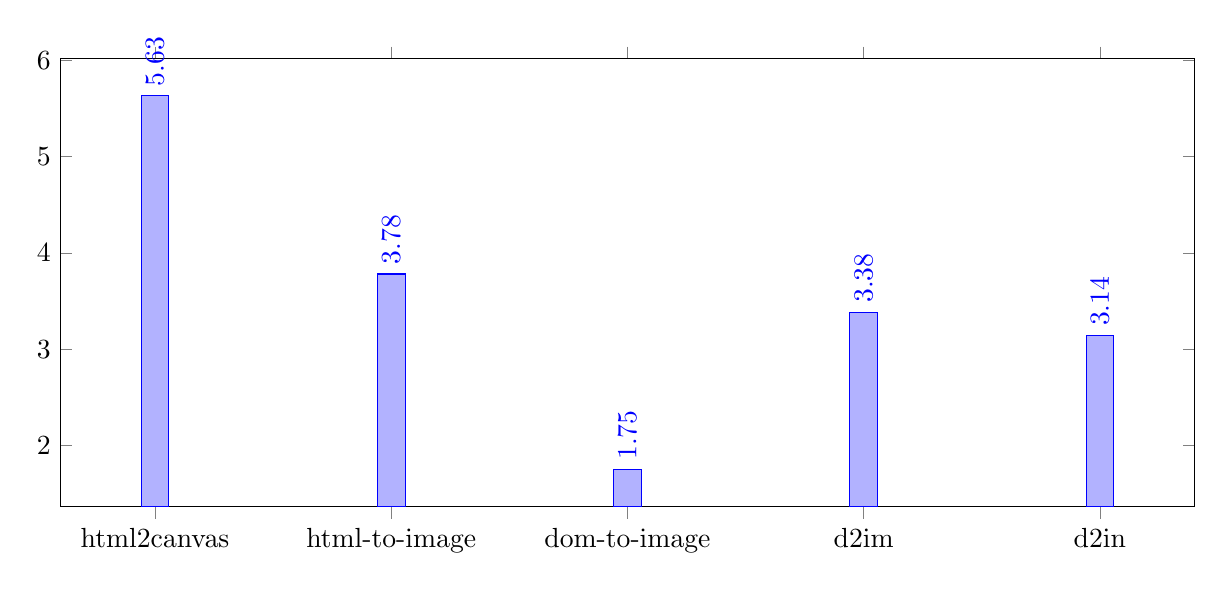
\begin{tikzpicture}
    \begin{axis}[
        ybar,
        x=3cm,
        symbolic x coords={html2canvas,html-to-image,dom-to-image,d2im,d2in},
        xtick=data,
        nodes near coords,
        every node near coord/.append style={
            rotate=90,
            anchor=west,
        }
    ]
    \addplot coordinates {(html2canvas, 5.63) (html-to-image, 3.78) (dom-to-image, 1.75) (d2im, 3.38) (d2in, 3.14)}; 
    \end{axis}
\end{tikzpicture}
\footnote{库名字过长无法渲染,请见脚注}
\footnote{d2im: dom-to-image-more}
\footnote{d2in: dom-to-image-next}
\p{
    可见还是html2canvas的性能最好。
}
.\\\\\textbf{线程池\\}
\p{
    既然无法提升渲染速度,那就试图将渲染内容放到别的地方去,不阻塞用户操作,同时新的页面也没有那么多元素,能提高复制解析的速度。
}
\p{
    考虑线程池,可以请求用户弹出几个窗口,将渲染任务轮流分配到这几个窗口上,如果窗口全部无法打开再在主线程中渲染。
}
\p{
    源代码请见\url{https://github.com/lihugang/mep2/commit/17668e040da9d8c776d5d3b872f3745567bf2f0c}
}
.\\\\
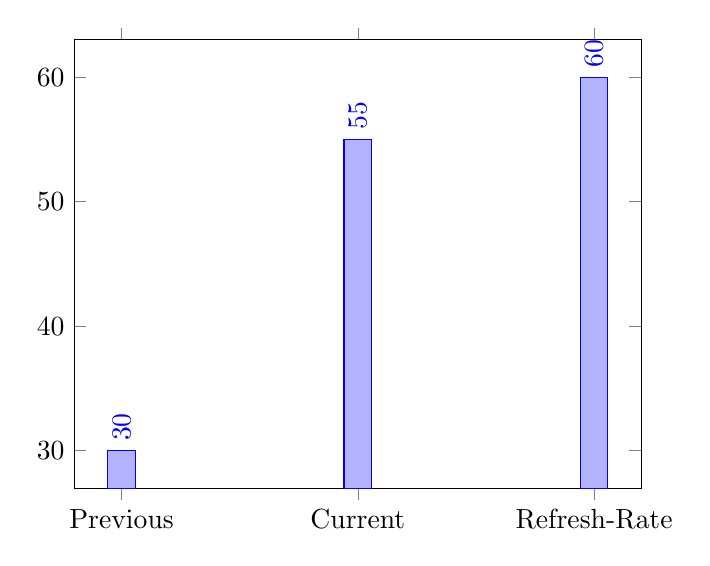
\begin{tikzpicture}
    \begin{axis}[
        ybar,
        x=3cm,
        symbolic x coords={Previous,Current,Refresh-Rate},
        xtick=data,
        nodes near coords,
        every node near coord/.append style={
            rotate=90,
            anchor=west,
        }
    ]
    \addplot coordinates {(Previous,30) (Current,55) (Refresh-Rate,60)}; 
    \end{axis}
\end{tikzpicture}
\p{
    如上图,在启用渲染线程池后,fps有很大提升,从30提升到55,逼近屏幕刷新率60。
}